\documentclass[a4paper,12pt]{article}
\usepackage[ margin=2cm ]{geometry}
\usepackage[utf8]{inputenc}
\usepackage[T1]{fontenc}
\usepackage[italian]{babel}
\usepackage{enumerate}
\usepackage{graphicx}
\usepackage{listings}

\title{Documentazione del protocollo di comunicazione}
\author{Leonardo Bianconi, Alexandru Gabriel Bradatan, Mattia Busso\\Gruppo 36}

\begin{document}

\maketitle
\tableofcontents

\section{Introduzione}

In questo documento verrà dettagliato il protocollo di comunicazione tra
client e server dell'implementazione di Eriantys del gruppo 36.

Il protocollo userà JSON e sarà codificato in UTF-8.

\section{Sequenza}

Distinguiamo 5 possibili scenari di interazione tra le parti:

\begin{enumerate}
\item Ricerca delle partite
\item Creazione di una nuova partita
\item Unione/abbandono di una partita
\item Fase di gioco
\item Ping
\end{enumerate}

Tranne per il ping, che è continuo dall'unione del giocatore fino alla fine
della partita, tutti gli scenari si svolgeranno nella sequenza con cui sono
stati indicati sopra.

\subsection{Ricerca delle partite}

Il client manderà una richiesta di tipo \texttt{FETCH} al server, il quale
risponderà con una lista delle lobby non ancora al completo in una risposta
di tipo \texttt{LOBBIES}.

\begin{figure}[htb]
  \centering
  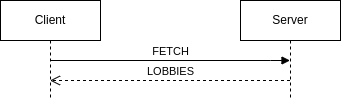
\includegraphics[width=10cm]{fetch.png}
  \caption{Scenario di ricerca delle partite}%
  \label{fig:fetch}
\end{figure}

\subsection{Creazione di una partita}

Se un giocatore volesse creare una nuova lobby, il client manderà al server
un messaggio di tipo \texttt{CREATE}. Il server risponderà con un messaggio
di tipo \texttt{UPDATE} che conterrà lo stato di default di una partita non
ancora inizializzata.

\begin{figure}[htb]
  \centering
  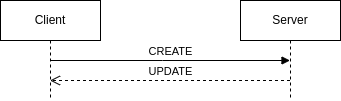
\includegraphics[width=10cm]{create.png}
  \caption{Scenario di creazione della partita}%
  \label{fig:create}
\end{figure}

\subsection{Unione/abbandono di una partita}

Se un giocatore volesse unirsi ad una lobby già esistente, il client manderà
al server un messaggio di tipo \texttt{JOIN}. Il server risponderà in
broadcast a tutti i client connessi alla stessa lobby con un messaggio di
tipo \texttt{UPDATE} contenente la nuova lista di giocatori e la nuova
plancia del giocatore appena unito.

Analogamente, nel caso in cui un giocatore volesse abbandonare la lobby, il
client manderà un messaggio di \texttt{LEAVE} e il server risponderà in
broadcast con un messaggio di \texttt{UPDATE} contenente la lista di
giocatori aggiornata. Al giocatore che sta lasciando la partita verrà mandato un
messaggio di \texttt{LEFT} come ACK dell'esecuzione della richiesta.

Nel caso di un eventuale crash del server, i client potranno riconnettersi alla
loro vecchia partita mandando dei messaggi di \texttt{JOIN} contenenti l'id
della vecchia partita e lo stesso username. Dopo che tutti i giocatori si
saranno uniti, la partita riprenderà.

Nota: la fase di \textit{lobby} di una partita è l'unico momento in cui un
giocatore ha la possibilità di unirsi e abbandonare la partita. Se un
giocatore si disconnette a partita già iniziata, la partita verrà terminata.

\begin{figure}[htb]
  \centering
  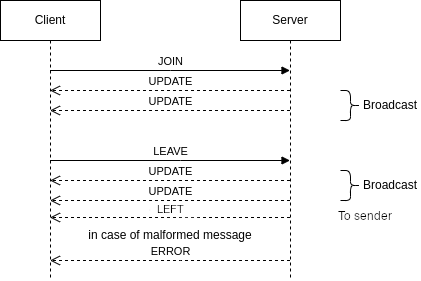
\includegraphics[width=10cm]{join.png}
  \caption{Scenario di unione ad una partita esistente}%
  \label{fig:join}
\end{figure}

\subsection{Fase di gioco}

La fase di gioco inizia non appena si uniscono tutti i giocatori. I client
manderanno dei comandi corrispondenti alle possibili azioni al server, il
quale risponderà con \texttt{UPDATE} in broadcast nel caso la modifica vada
a buon fine o con un \texttt{ERROR} diretto al mittente in caso di azione
non permessa o messaggio malformato.

Nel caso un comando causi la fine della partita, un messaggio di
\texttt{END} verrà mandato in broadcast contente la lista dei vincitori della
partita.

\begin{figure}[htb]
  \centering
  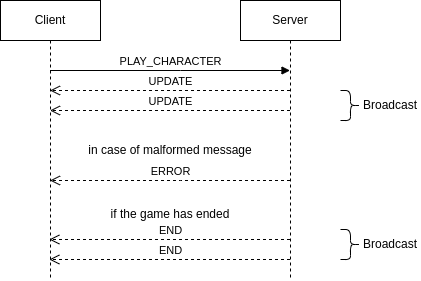
\includegraphics[width=10cm]{game.png}
  \caption{Scenario di gioco, in questo esempio con un comando per giocare un personaggio}%
  \label{fig:game}
\end{figure}

\subsection{Ping}

Durante tutta la connessione ad una partita, il server manderà un messaggio
di \texttt{PING} ai vari client ad intervalli regolari. A questi messaggi i
client risponderanno con il corrispondente \texttt{PONG}.

Se un client non risponde in tempo al ping, il server terminerà la partita
di cui fa parte e manderà un messaggio di \texttt{END} in broadcast agli
altri membri della partita.

\begin{figure}[htb]
  \centering
  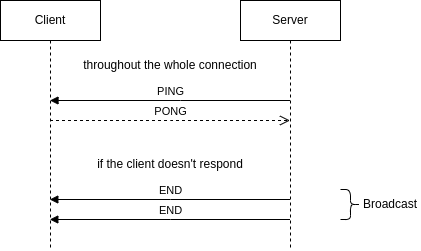
\includegraphics[width=10cm]{ping.png}
  \caption{Ping tra server e client}%
  \label{fig:ping}
\end{figure}

\subsection{Esempio di partita}

In figura~\ref{fig:example} verrà riportato uno scambio di esempio tra un
client ed il server. Un giocatore, dopo aver scelto una partita dalla lista
di partite disponibili vi si unisce. In seguito prova ad usare l'effetto di
una carta personaggio in un momento non consentito; la mossa successiva,
però, è legittima. Infine il server conclude la partita a causa della
vittoria di un giocatore. Per chiarezza del diagramma i messaggi di ping
sono stati omessi.

\begin{figure}[htb]
  \centering
  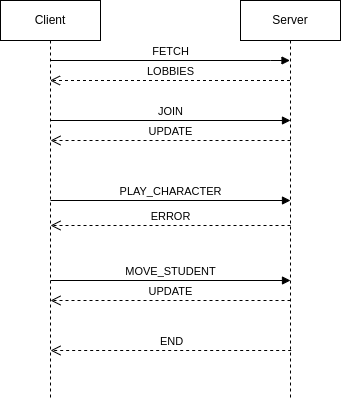
\includegraphics[width=10cm]{example.png}
  \caption{Scambio d'esempio}%
  \label{fig:example}
\end{figure}

\newpage

\section{Dettaglio messaggi client}

In questa sezione verranno descritti tramite degli esempi i vari messaggi
inviati dai client al server

\subsection{\texttt{FETCH}}

Richiede una lista di partite libere al server.

\begin{verbatim}
{
  "type": "FETCH"
}
\end{verbatim}

\subsection{\texttt{CREATE}}

Richiede la creazione di una nuova lobby con i parametri indicati. Il
giocatore che crea la lobby vi è automaticamente aggiunto.

\begin{verbatim}
{
  "username": "ann",
  "type": "CREATE",
  "arguments": [
    {
      "nPlayers": 2
      "expert": true
    }
  ]
}
\end{verbatim}

\subsection{\texttt{JOIN} e \texttt{LEAVE}}

Rispettivamente richiedono l'aggiunta o la rimozione del giocatore con lo
username specificato all partita  con l'identificativo dato.

\begin{verbatim}
{
  "gameId": 1234567890,
  "username": "ann",
  "type": "JOIN"
}

{
  "gameId": 1234567890,
  "username": "ann",
  "type": "LEAVE"
}
\end{verbatim}

\subsection{Comandi di gioco}

Questa serie di comandi rappresentano le varie mosse eseguibili da un
giocatore durante una partita, come ad esempio il movimento degli studenti
o di madre natura. Ogni comando possiede l'identificativo della partita a cui
appartiene, lo username del giocatore che lo esegue, il tipo di comando e
una lista di parametri variabile in base al tipo di comando.

Per scopi documentativi, sono stati aggiunti dei commenti delimitati da
\texttt{//}.

\begin{verbatim}
{
  "gameId": 1234567890,
  "username": "ann",
  "type": "CHOOSE_MAGE",
  "arguments": ["WIZARD"] // valori dall'enum Mage
}

{
  "gameId": 1234567890,
  "username": "ann",
  "type": "PLAY_ASSISTANTS",
  "arguments": ["CAT"] // valori dall'enum AssistantType
}

{
  "gameId": 1234567890,
  "username": "ann",
  "type": "MOVE_STUDENT",
  // Solo uno dei seguenti oggetti sarà mai mandato, sono stati riportati
  // entrambi per scopi documentativi
  "arguments": [
    {
      "destination": "HALL",
      "color": "RED" // valore dall'enum PieceColor
    },
    {
      "destination": "ISLAND",
      "color": "RED", // valore dall'enum PieceColor
      "index": 0
    }
  ]
}

{
  "gameId": 1234567890,
  "username": "ann",
  "type": "PLAY_CHARACTER",
  "arguments": [
    {
      "character": "PRIEST", // Valore dall'enum CharacterType
      "steps": [
        {
          "key1": "value1",
          "key2": "value2"
        },
        {
          "key1": "value1",
          "key2": "value2"
        }
      ]
    }
  ]
}

{
  "gameId": 1234567890,
  "username": "ann",
  "type": "MOVE_MN",
  "arguments": [3] // Numero di isole di cui si vuole muovere madre natura
}

{
  "gameId": 1234567890,
  "username": "ann",
  "type": "PICK_CLOUD",
  "arguments": [2] // Id della nuvola che si vuole prendere
}
\end{verbatim}

\subsection{\texttt{PONG}}

\begin{verbatim}
{
  "gameId": 1234567890
  "type": "PONG"
}
\end{verbatim}

\section{Dettaglio messaggi server}

In questa sezione verranno descritti tramite degli esempi i vari messaggi
inviati dal server ai client.

\subsection{\texttt{LOBBIES}}

Questa risposta è mandata in seguito ad un comando di \texttt{FETCH}. Essa
contiene una lista di tutte le lobby che non sono ancora piene, con le
relative caratteristiche.

\begin{verbatim}
{
  "type": "LOBBIES"
  "lobbies": [
    {
      "id": 1234567890,
      "nPlayers": 2,
      "expert": true,
      "playersConnected": 1, // Il numero di giocatori attualmente connessi
      "rejoining": true // true solo se la partita è in attesa dei giocatori
                        // che è stata ripristinata da disco.
                        // Se la partita è stata avviata normalmente il valore
                        // sarà false o sarà omesso del tutto.
    }
  ]
}
\end{verbatim}

\subsection{\texttt{UPDATE}}

Risposta di successo mandata in seguito ad un comando che modifica lo stato
del gioco. Contiene tutti e soli gli oggetti modificati dal comando a cui è
risposta. Nell'esempio riportato in seguito è stata riportata la massima
estensione del comando.

\begin{verbatim}
{
  "id": 1234567890,
  "type": "UPDATE",
  "rejoining": true, // vedasi "rejoining" di LOBBIES
  "missingPlayers": 2 // presente solo se  rejoining == true, indica il numero
                      // di giocatori che devono ancora riconnettersi affinchè
                      // la partita riprenda
  "update": {
    "phase": "PhaseName",
    "currentPlayer": "ann",
    "playerList": ["ann", "bob"],
    "professors": [
      {
        "color": "RED",
        "owner": "bob"
      }
    ],
    "boards": [
      {
        "username": "ann",
        "entrance": ["RED", "BLUE"],
        "assistants": ["CAT"],
        "lastPlayedAssistant": "ELEPHANT",
        "hall": ["RED", "BLUE"],
        "towers": ["BLACK", "BLACK"],
        "coins": 5
      }
    ],
    "islandList": [[0], [1,2,3], [4,5,6], [7,8,9,10,11]],
    "islands": [
      {
        "ids": [1,2,3],
        "students": ["RED", "BLUE"],
        "towers": ["BLACK", "BLACK", "BLACK"],
        "blocks": 2
      }
    ],
    "motherNature": 10,
    "usedCharacter": false,
    "characters": [
      {
        "type": "PRIEST",
        "students": ["RED", "BLUE"],
        "price": 3,
      }
    ],
    "isSackEmpty": false,
    "clouds": [
      {
        "id": 1,
        "students": []
      }
    ]
  }
}
\end{verbatim}

\subsection{\texttt{END}}

La risposta di tipo \texttt{END} viene mandata al posto di un
\texttt{UPDATE} se il comando ricevuto ha causato la fine del gioco. La
risposta di \texttt{END} viene anche mandata per segnalare la terminazione
del gioco in caso di disconnessione di un giocatore.

\begin{verbatim}
{
  "id": 1234567890,
  "type": "END",
  "winners": ["ann"]
  "reason": "A winner has been found"
}

{
  "id": 1234567890,
  "type": "END",
  "winners": []
  "reason": "A player has disconnected"
}
\end{verbatim}

\subsection{\texttt{LEFT}}

La risposta di tipo \texttt{LEFT} viene mandata ad un giocatore che ha mandato
una richiesta di \texttt{LEAVE} che è stata processata correttamente.

\begin{verbatim}
{
  "id": 1234567890,
  "type: "LEFT"
}
\end{verbatim}

\subsection{\texttt{ERROR}}

Mandato in risposta ad un comando malformato o non permesso in quel momento
della partita in corso.

\begin{verbatim}
{
  "id": 1234567890,
  "type": "ERROR",
  "reason": "This action is not allowed now"
}
\end{verbatim}

\subsection{\texttt{PING}}

\begin{verbatim}
{
  "id": 1234567890,
  "type": "PING"
}
\end{verbatim}

\end{document}
